\documentclass[a4paper, 12pt]{article}
\usepackage{temp}
\usepackage{epsfig,graphicx,subfigure,amsthm,amsmath, float, xcolor, changepage, mathtools, textcomp, hyperref, bm, amssymb, tcolorbox, tikz, setspace}
\usepackage{array}
\usepackage[shortlabels]{enumitem}
\usepackage[bottom]{footmisc}
\usepackage{xepersian}
\settextfont[Scale=1]{XBZar}
%\setdigitfont{XBZar}
\setlatintextfont[Scale=0.9]{Times New Roman}
\hypersetup{
	colorlinks=true,
	urlcolor=blue!70!black
}

\newcolumntype{?}{!{\vrule width 1pt}}

\doublespacing
\begin{document}
\handout
{هوش مصنوعی}
{نیم‌سال اول
۱۴۰۱\lr{-}۱۴۰۰}
{دکتر محمدحسین رهبان}
{دانشکده مهندسی کامپیوتر}
{مینی‌پروژه دوم - تئوری}
{محمدجواد هزاره}
{98101074}
\noindent
\\[-6em]
\section*{سوال ۱}
\begin{enumerate}[A)]
	\item \textbf{نادرست}؛
	اگر طول گام به اندازه‌ی کافی کوتاه انتخاب نشود، الگوریتم لزوما همگرا نخواهد شد؛ چرا که با گام بلند به مکان بسیار دوری از موضع فعلی منتقل خواهیم شد و اطلاعی از آن مکان نداریم. در مکان فعلی به صورت موضعی انتظار داریم گرادیان زیاد تغییر نکند پس با گام‌های کوتاه در جهت خلاف گرادیان می‌توان به صورت پیوسته به سمت نقطه کمینه حرکت کرد.
	\item \textbf{درست}؛
	اگر الگوریتم $x = x^\prime$ را ببیند، از آن‌جایی که
	$f^\prime(x^\prime) = 0$،
	در این نقطه باقی خواهد ماند و هرگز به 
	$x^\ast$
	نخواهد رسید.
	\item \textbf{نادرست}؛
	قسمت «اگر» در گزاره‌ی داده شده صحیح است. اگر تابع $f$ محدب باشد و الگوریتم همگرا شود، به نقطه کمینه سراسری که همان $x^\ast$ است همگرا خواهد شد. اما قسمت «تنها اگر» درست نیست. اگر الگوریتم همگرا شده و به $x^\ast$ برسد، الزامی وجود ندارد که تابع $f$ محدب باشد. ممکن است از نقطه‌ای شروع کنیم که نزدیک $x^\ast$ بوده و در جایی دورتر از این نقطه تابع $f$ محدب نباشد.
	\item \textbf{درست}؛
	مشتق دوم تابع داده شده برابر $w$ است و از آن‌جایی که می‌دانیم تابع باید کمینه داشته باشد، $w$ مقداری مثبت خواهد داشت. با توجه به مثبت بودن $w$ تابع محدب است و درنتیجه در صورت همگرایی الگوریتم، به $x^\ast$ همگرا خواهد شد.
\end{enumerate}
\section*{سوال ۲}
\begin{enumerate}[A)]
	\item
	در هر سه حالت نیازی به \lr{backtrack} نیست. با توجه به تعریف \lr{consistent} بودن یال‌ها، هر سه ترتیب بدون بازگشت راس‌ها را مقداردهی می‌کنند.
	\item
	ترتیب
	$\{A,D,B,G,E,H,C,F\}$
	حداکثر دو بازگشت خواهد داشت. چرا که فقط وقتی به متغیر‌های $C$ و $F$ می‌رسیم، دو یا چند متغیر دیگر که به آن‌ها متصل هستند مقداردهی شده‌اند و ممکن است مقداردهی‌ای برای این متغیرها وجود نداشته باشد که با مقداردهی‌های قبلی سازگار باشد. بنابراین در این دو متغیر امکان بازگشت وجود دارد. با همین استدلال می‌توان سایر ترتیب‌ها را رد کرد.
	\item
\end{enumerate}
\section*{سوال ۳}
در این حالت که هیچ قیدی روی مقدار برگ‌ها نداریم، فقط سمت راست‌ترین برگ می‌تواند هرس شود.
\begin{figure}[H]
	\centering
	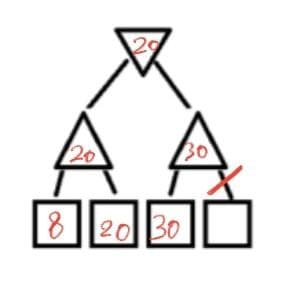
\includegraphics[width=.3\textwidth]{3-1.jpg}
\end{figure}
\begin{enumerate}[A)]
	\item
	در این حالت که هیچ قیدی روی مقادیر برگ‌ها نداریم، با وجود گره‌های \lr{expectimax} حتما همه‌ی مقادیر برگ‌ها را باید ببینیم. به عبارتی هیچ برگی هرس نخواهد شد.
	\item
	برای حالتی که گره بیشینه داریم، حالات مختلفی وجود دارد که در تصاویر زیر آمده است.
	\begin{figure}[H]
		\centering
		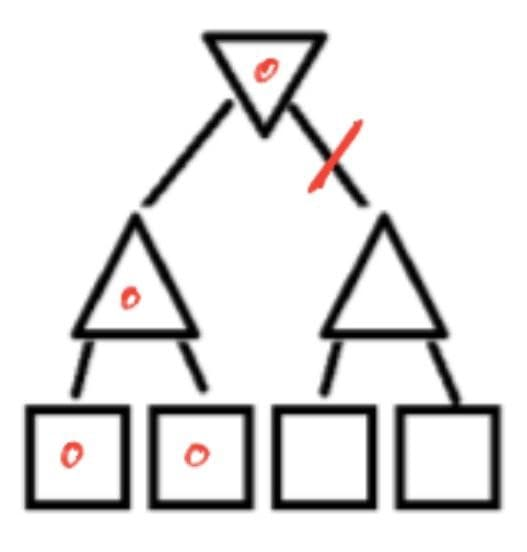
\includegraphics[width=.24\textwidth]{3-2-1.jpg} \vline
		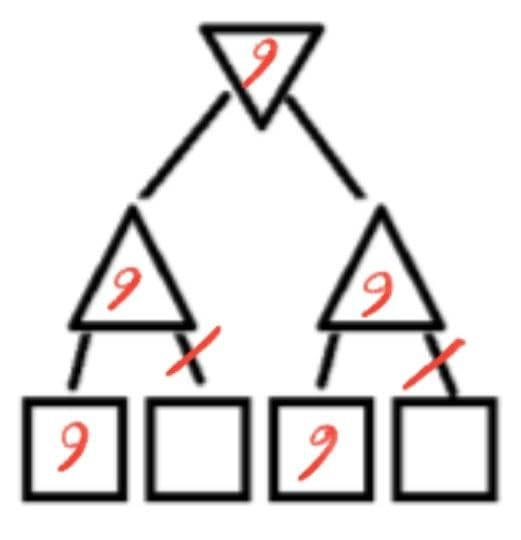
\includegraphics[width=.24\textwidth]{3-2-2.jpg} \vline
		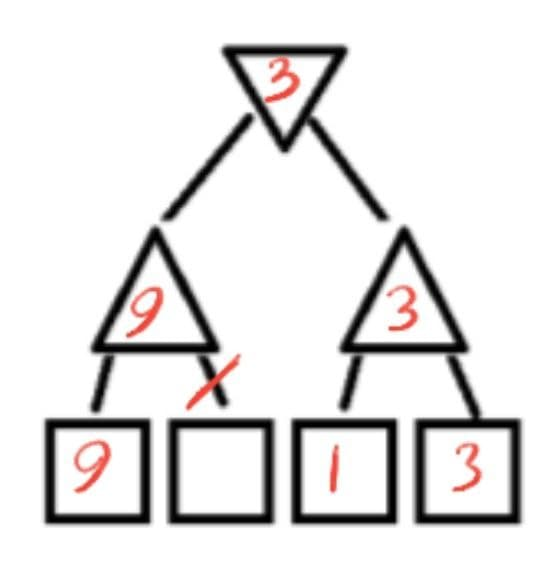
\includegraphics[width=.24\textwidth]{3-2-3.jpg} \vline
		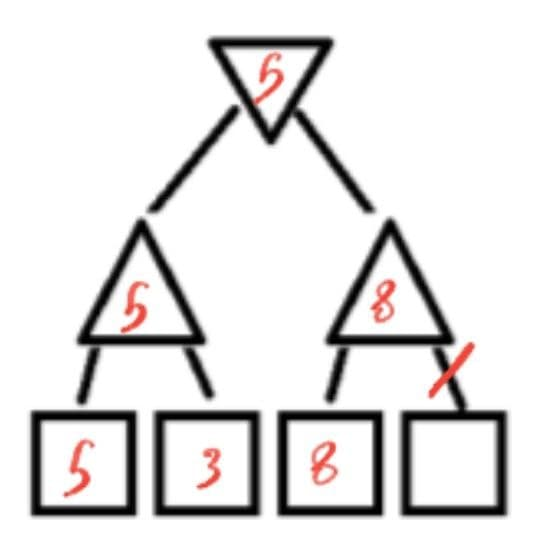
\includegraphics[width=.24\textwidth]{3-2-4.jpg}
	\end{figure}
	و برای حالتی که گره \lr{expectimax} داریم نیز به صورت زیر خواهد بود.
	\begin{figure}[H]
		\centering
		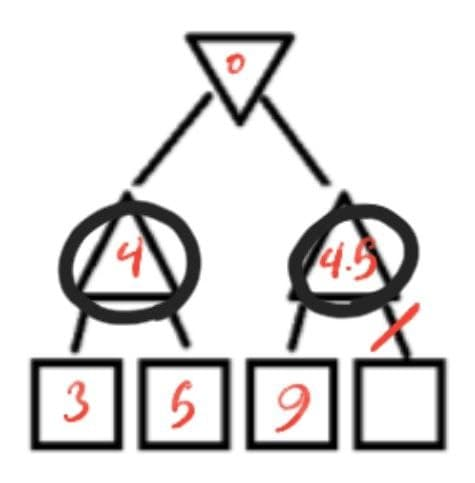
\includegraphics[width=.24\textwidth]{3-3-1.jpg} \vline
		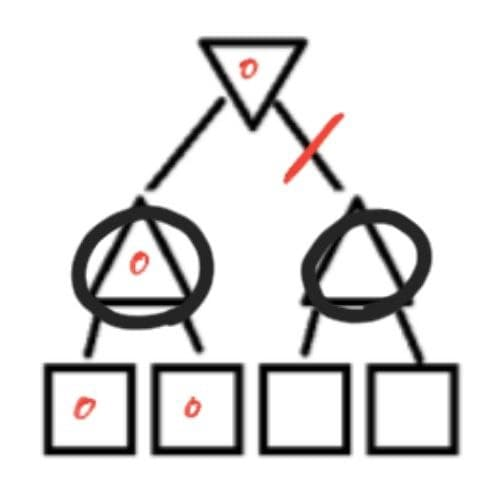
\includegraphics[width=.24\textwidth]{3-3-2.jpg}
	\end{figure}
\end{enumerate}
\end{document}



